\section{Tikz}

\subsection{tikzpicture}

\subsubsection{Un grafico base}

\begin{verbatim}
    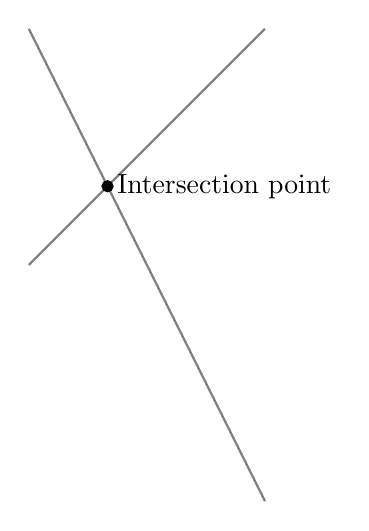
\begin{tikzpicture}
        \draw[gray, thick] (-1,2) -- (2,-4);
        \draw[gray, thick] (-1,-1) -- (2,2);
        \filldraw[black] (0,0) circle (2pt) node[anchor=west] {Intersection point};
    \end{tikzpicture}
\end{verbatim}

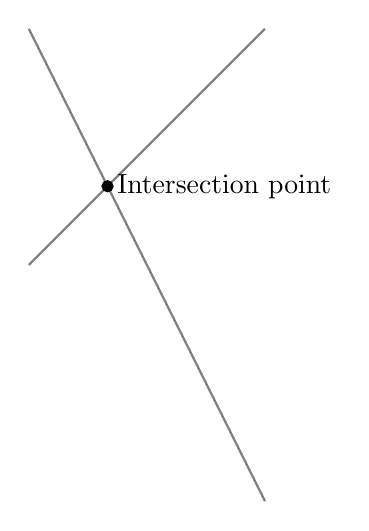
\begin{tikzpicture}
\draw[gray, thick] (-1,2) -- (2,-4);
\draw[gray, thick] (-1,-1) -- (2,2);
\filldraw[black] (0,0) circle (2pt) node[anchor=west] {Intersection point};
\end{tikzpicture}

\subsubsection{Albero MergeSort}

Per avere controllo sulle posizioni:

\begin{verbatim}
[level distance=1.5cm,
level 1/.style={sibling distance=3.5cm},
level 2/.style={sibling distance=1cm}]
\end{verbatim}

\begin{verbatim}
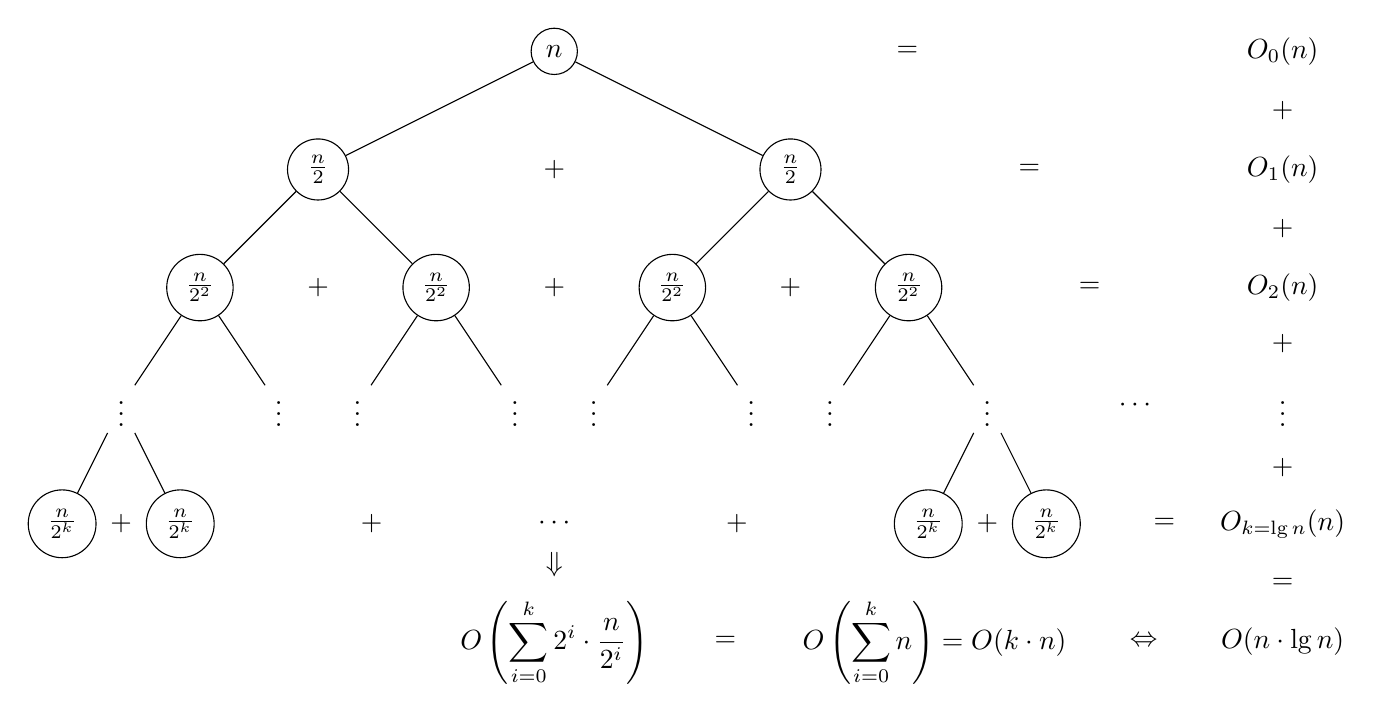
\begin{tikzpicture}[level/.style={sibling distance=60mm/#1}]
\node [circle,draw] (z){$n$}
  child {node [circle,draw] (a) {$\frac{n}{2}$}
    child {node [circle,draw] (b) {$\frac{n}{2^2}$}
      child {node {$\vdots$}
        child {node [circle,draw] (d) {$\frac{n}{2^k}$}}
        child {node [circle,draw] (e) {$\frac{n}{2^k}$}}
      } 
      child {node {$\vdots$}}
    }
    child {node [circle,draw] (g) {$\frac{n}{2^2}$}
      child {node {$\vdots$}}
      child {node {$\vdots$}}
    }
  }
  child {node [circle,draw] (j) {$\frac{n}{2}$}
    child {node [circle,draw] (k) {$\frac{n}{2^2}$}
      child {node {$\vdots$}}
      child {node {$\vdots$}}
    }
  child {node [circle,draw] (l) {$\frac{n}{2^2}$}
    child {node {$\vdots$}}
    child {node (c){$\vdots$}
      child {node [circle,draw] (o) {$\frac{n}{2^k}$}}
      child {node [circle,draw] (p) {$\frac{n}{2^k}$}
        child [grow=right] {node (q) {$=$} edge from parent[draw=none]
          child [grow=right] {node (q) {$O_{k = \lg n}(n)$} edge from parent[draw=none]
            child [grow=up] {node (r) {$\vdots$} edge from parent[draw=none]
              child [grow=up] {node (s) {$O_2(n)$} edge from parent[draw=none]
                child [grow=up] {node (t) {$O_1(n)$} edge from parent[draw=none]
                  child [grow=up] {node (u) {$O_0(n)$} edge from parent[draw=none]}
                }
              }
            }
            child [grow=down] {node (v) {$O(n \cdot \lg n)$}edge from parent[draw=none]}
          }
        }
      }
    }
  }
};
\path (a) -- (j) node [midway] {+};
\path (b) -- (g) node [midway] {+};
\path (k) -- (l) node [midway] {+};
\path (k) -- (g) node [midway] {+};
\path (d) -- (e) node [midway] {+};
\path (o) -- (p) node [midway] {+};
\path (o) -- (e) node (x) [midway] {$\cdots$}
  child [grow=down] {
    node (y) {$O\left(\displaystyle\sum_{i = 0}^k 2^i \cdot \frac{n}{2^i}\right)$}
    edge from parent[draw=none]
  };
\path (q) -- (r) node [midway] {+};
\path (s) -- (r) node [midway] {+};
\path (s) -- (t) node [midway] {+};
\path (s) -- (l) node [midway] {=};
\path (t) -- (u) node [midway] {+};
\path (z) -- (u) node [midway] {=};
\path (j) -- (t) node [midway] {=};
\path (y) -- (x) node [midway] {$\Downarrow$};
\path (v) -- (y)
  node (w) [midway] {$O\left(\displaystyle\sum_{i = 0}^k n\right) = O(k \cdot n)$};
\path (q) -- (v) node [midway] {=};
\path (e) -- (x) node [midway] {+};
\path (o) -- (x) node [midway] {+};
\path (y) -- (w) node [midway] {$=$};
\path (v) -- (w) node [midway] {$\Leftrightarrow$};
\path (r) -- (c) node [midway] {$\cdots$};
\end{tikzpicture}
\end{verbatim}
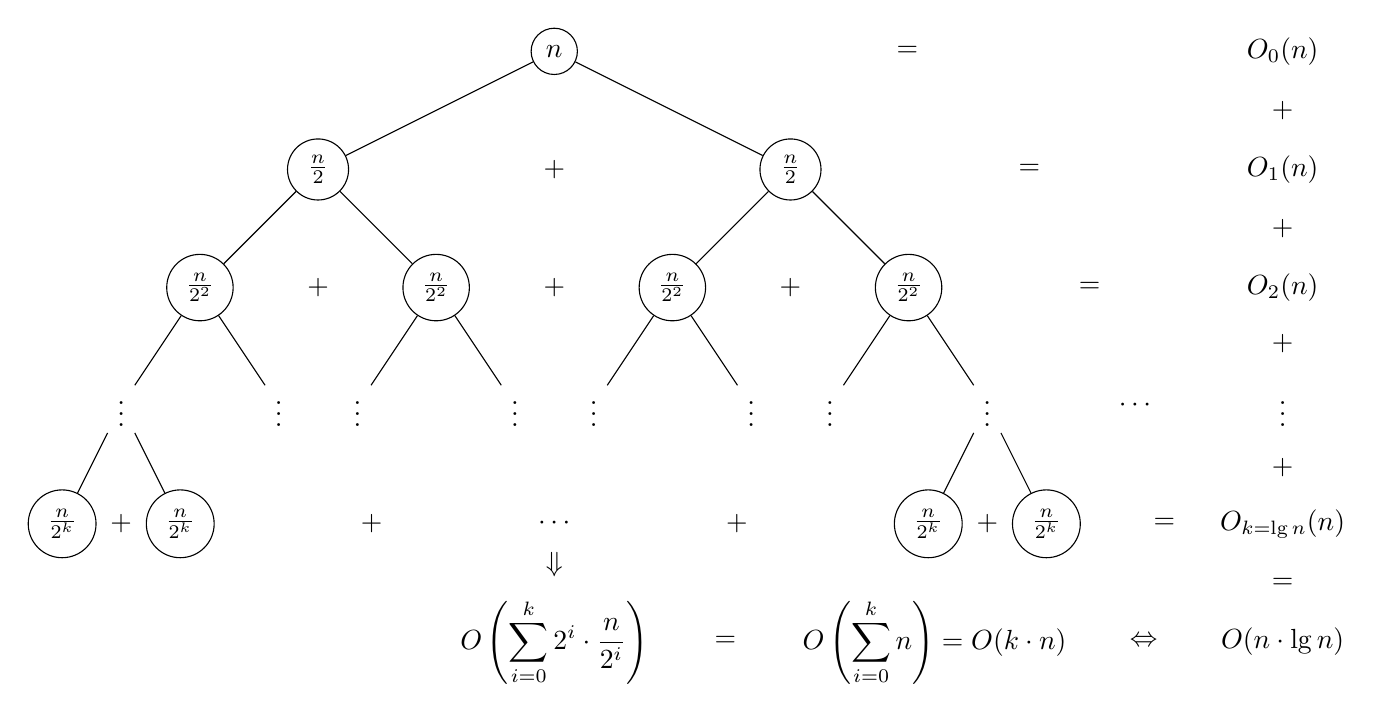
\begin{tikzpicture}[level/.style={sibling distance=60mm/#1}]
\node [circle,draw] (z){$n$}
  child {node [circle,draw] (a) {$\frac{n}{2}$}
    child {node [circle,draw] (b) {$\frac{n}{2^2}$}
      child {node {$\vdots$}
        child {node [circle,draw] (d) {$\frac{n}{2^k}$}}
        child {node [circle,draw] (e) {$\frac{n}{2^k}$}}
      } 
      child {node {$\vdots$}}
    }
    child {node [circle,draw] (g) {$\frac{n}{2^2}$}
      child {node {$\vdots$}}
      child {node {$\vdots$}}
    }
  }
  child {node [circle,draw] (j) {$\frac{n}{2}$}
    child {node [circle,draw] (k) {$\frac{n}{2^2}$}
      child {node {$\vdots$}}
      child {node {$\vdots$}}
    }
  child {node [circle,draw] (l) {$\frac{n}{2^2}$}
    child {node {$\vdots$}}
    child {node (c){$\vdots$}
      child {node [circle,draw] (o) {$\frac{n}{2^k}$}}
      child {node [circle,draw] (p) {$\frac{n}{2^k}$}
        child [grow=right] {node (q) {$=$} edge from parent[draw=none]
          child [grow=right] {node (q) {$O_{k = \lg n}(n)$} edge from parent[draw=none]
            child [grow=up] {node (r) {$\vdots$} edge from parent[draw=none]
              child [grow=up] {node (s) {$O_2(n)$} edge from parent[draw=none]
                child [grow=up] {node (t) {$O_1(n)$} edge from parent[draw=none]
                  child [grow=up] {node (u) {$O_0(n)$} edge from parent[draw=none]}
                }
              }
            }
            child [grow=down] {node (v) {$O(n \cdot \lg n)$}edge from parent[draw=none]}
          }
        }
      }
    }
  }
};
\path (a) -- (j) node [midway] {+};
\path (b) -- (g) node [midway] {+};
\path (k) -- (l) node [midway] {+};
\path (k) -- (g) node [midway] {+};
\path (d) -- (e) node [midway] {+};
\path (o) -- (p) node [midway] {+};
\path (o) -- (e) node (x) [midway] {$\cdots$}
  child [grow=down] {
    node (y) {$O\left(\displaystyle\sum_{i = 0}^k 2^i \cdot \frac{n}{2^i}\right)$}
    edge from parent[draw=none]
  };
\path (q) -- (r) node [midway] {+};
\path (s) -- (r) node [midway] {+};
\path (s) -- (t) node [midway] {+};
\path (s) -- (l) node [midway] {=};
\path (t) -- (u) node [midway] {+};
\path (z) -- (u) node [midway] {=};
\path (j) -- (t) node [midway] {=};
\path (y) -- (x) node [midway] {$\Downarrow$};
\path (v) -- (y)
  node (w) [midway] {$O\left(\displaystyle\sum_{i = 0}^k n\right) = O(k \cdot n)$};
\path (q) -- (v) node [midway] {=};
\path (e) -- (x) node [midway] {+};
\path (o) -- (x) node [midway] {+};
\path (y) -- (w) node [midway] {$=$};
\path (v) -- (w) node [midway] {$\Leftrightarrow$};
\path (r) -- (c) node [midway] {$\cdots$};
\end{tikzpicture}

% \begin{tikzpicture}[level/.style={sibling distance=60mm/#1}]
\begin{tikzpicture}[level/.style={sibling distance=40mm}]
    \node [draw, label=right:{Testo $math$}] (z){$n = f^{(0)}(n)$}
        child { node [ellipse,draw] (a) {$a f^{(0)}(n)$}
            child { node [circle,draw] (c) {$c f^{(0)}(n)$}
            }
            child { node [rectangle,draw] (d) {$d f^{(0)}(n)$}
                child { node [rectangle,draw] (e) {$e f^{(0)}(n)$}
                }
                child { node [rectangle,draw] (f) {$f f^{(0)}(n)$}
                }
            }
        }
        child { node [circle,draw] (b) {$b f^{(0)}(n)$}
        }
        % child [grow=right] {node (q) {$O_{k = \lg n}(n)$} edge from parent[draw=none]
        % }
    ;
\path (a) -- (b) node [midway] {$\cdots S(n) \cdots$ };
\end{tikzpicture}


\section{pgfplots}

Pgfplots can do basically any plot, more info \href{https://it.overleaf.com/learn/latex/Pgfplots_package}{here}







\subsubsection{Un grafico esponenziale}

\begin{verbatim}
\begin{tikzpicture}
    \begin{axis}
        \addplot[color=red]{exp(x)};
    \end{axis}
\end{tikzpicture}
%Here ends the furst plot
\hskip 5pt
%Here begins the 3d plot
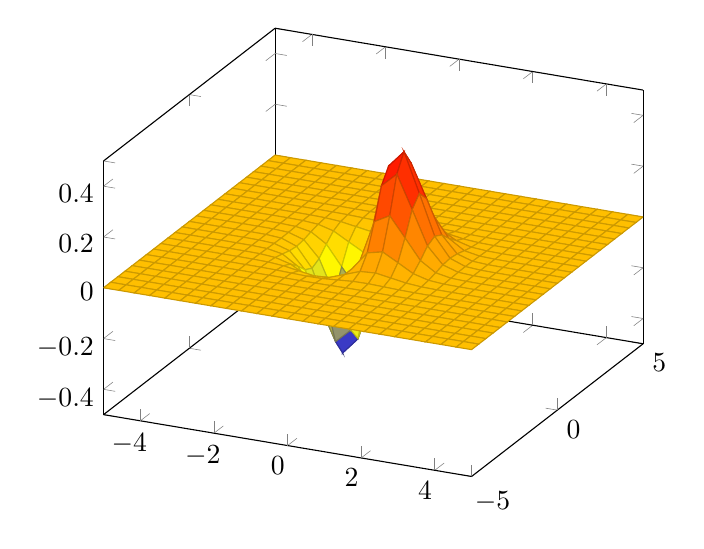
\begin{tikzpicture}
    \begin{axis}
        \addplot3[
                surf,
            ]
        {exp(-x^2-y^2)*x};
    \end{axis}
\end{tikzpicture}
\end{verbatim}

\begin{tikzpicture}
    \begin{axis}
        \addplot[color=red]{exp(x)};
    \end{axis}
\end{tikzpicture}
%Here ends the furst plot
% \hskip 5pt
%Here begins the 3d plot
% \begin{tikzpicture}
    % \begin{axis}
        % \addplot3[
                % surf,
            % ]
        % {exp(-x^2-y^2)*x};
    % \end{axis}
% \end{tikzpicture}

\subsection{2D plots}

\begin{verbatim}
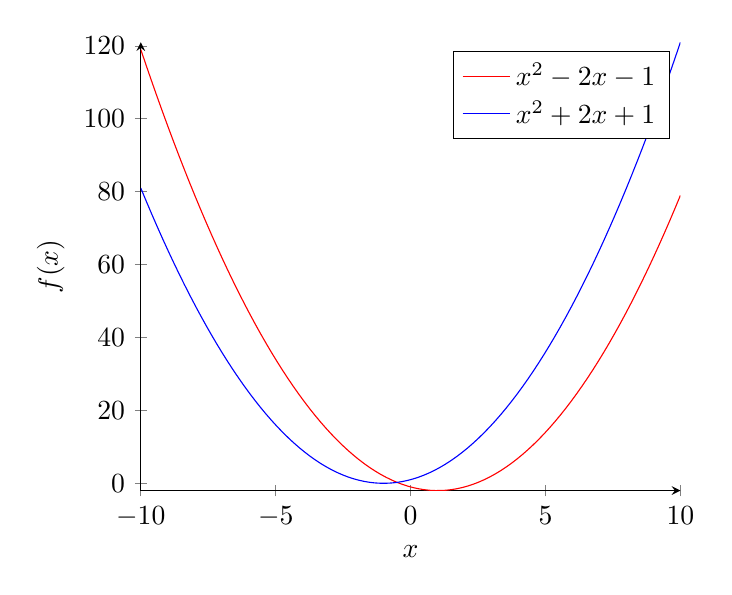
\begin{tikzpicture}
\begin{axis}[
    axis lines = left,
    xlabel = $x$,
    ylabel = {$f(x)$},
]
%Below the red parabola is defined
\addplot [
    domain=-10:10, 
    samples=100, 
    color=red,
]
{x^2 - 2*x - 1};
\addlegendentry{$x^2 - 2x - 1$}
%Here the blue parabloa is defined
\addplot [
    domain=-10:10, 
    samples=100, 
    color=blue,
    ]
    {x^2 + 2*x + 1};
\addlegendentry{$x^2 + 2x + 1$}
 
\end{axis}
\end{tikzpicture}
\end{verbatim}
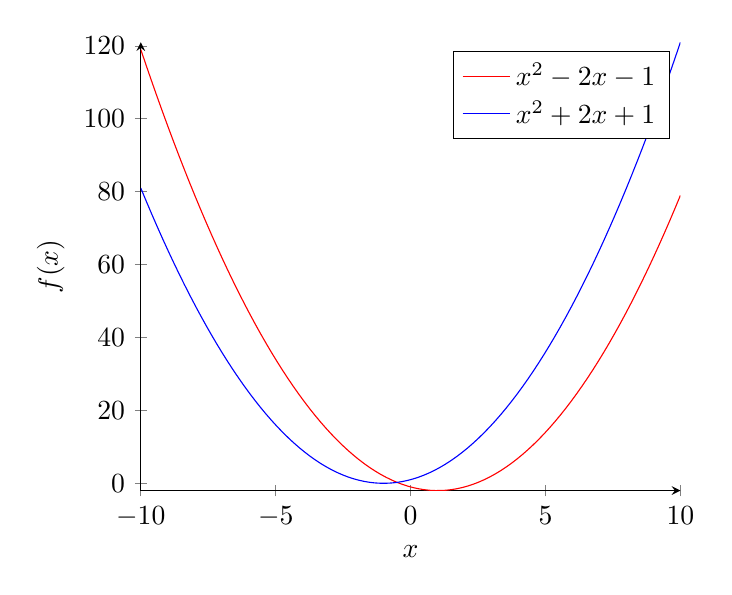
\begin{tikzpicture}
\begin{axis}[
    axis lines = left,
    xlabel = $x$,
    ylabel = {$f(x)$},
]
%Below the red parabola is defined
\addplot [
    domain=-10:10, 
    samples=100, 
    color=red,
]
{x^2 - 2*x - 1};
\addlegendentry{$x^2 - 2x - 1$}
%Here the blue parabloa is defined
\addplot [
    domain=-10:10, 
    samples=100, 
    color=blue,
    ]
    {x^2 + 2*x + 1};
\addlegendentry{$x^2 + 2x + 1$}
 
\end{axis}
\end{tikzpicture}
